\documentclass[12pt,a4paper]{report}

% ------------------------------------------------------------------
% DRL-VNE for SAGIN - Major Project Report
% SIT, Tumakuru template  |  Overleaf-ready (no external files needed)
% Compile with pdfLaTeX.
% ------------------------------------------------------------------
\usepackage{xcolor}
\usepackage[utf8]{inputenc}
\usepackage[T1]{fontenc}
\usepackage{graphicx}
\usepackage{amsmath,amssymb}
\usepackage{booktabs}
\usepackage{array}
\usepackage{tabularx}
\usepackage{float}
\usepackage{longtable}
\usepackage{geometry}
\usepackage{setspace}
\usepackage{times}
\usepackage{fancyhdr}
\usepackage{titlesec}
\usepackage[hidelinks]{hyperref}
\usepackage{caption}
\usepackage{enumitem}
\usepackage{algorithm}
\usepackage{algpseudocode}
\usepackage{tikz}           % for the logo placeholder box

\geometry{left=1.3in,right=1in,top=1in,bottom=1in}
\onehalfspacing

% ------------------------------------------------------------------
% Logo helper: draws a simple framed "SIT" badge so the layout
% matches the original template even without the actual image file.
% Replace \sitlogo with \includegraphics[width=0.18\textwidth]{sit_logo.png}
% once you upload the real logo to Overleaf.
% ------------------------------------------------------------------
\newcommand{\sitlogo}{%
  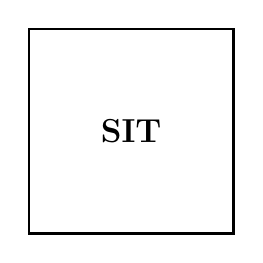
\begin{tikzpicture}
    \draw[thick] (0,0) rectangle (2.6,2.6);
    \node[font=\large\bfseries] at (1.3,1.3) {SIT};
  \end{tikzpicture}%
}

% Header / footer
\pagestyle{fancy}
\fancyhf{}
\lhead{DRL-VNE for SAGIN}
\rhead{2026--27}
\rfoot{Dept.\ of ISE, S.I.T., Tumakuru-03}
\lfoot{\thepage}
\renewcommand{\headrulewidth}{0.4pt}

\titleformat{\chapter}[display]
  {\normalfont\huge\bfseries}{\chaptertitlename\ \thechapter}{20pt}{\Huge}

% ------------------------------------------------------------------
\begin{document}

% ==================================================================
% TITLE PAGE
% ==================================================================
\begin{titlepage}
\centering
{\large\textbf{SIDDAGANGA INSTITUTE OF TECHNOLOGY, TUMAKURU-572103}}\\[2pt]
{\small (An Autonomous Institute under Visvesvaraya Technological University, Belagavi)}\\[24pt]

{\large Major Project Report}\\[4pt]
{\large on}\\[10pt]

{\Large\textbf{``DRL-VNE for SAGIN: Deep Reinforcement Learning based Virtual Network
Embedding over Space-Air-Ground Integrated Networks''}}\\[20pt]

{\normalsize submitted in partial fulfillment of the completion of VII semester of}\\[4pt]
{\large\textbf{BACHELOR OF ENGINEERING}}\\[4pt]
{\normalsize in}\\[4pt]
{\large\textbf{INFORMATION SCIENCE \& ENGINEERING}}\\[18pt]

{\normalsize Submitted by}\\[8pt]
{\large Avish Chawla \quad (1SI23IS009)}\\
{\large Mahashewata Ghosh \quad (1SI23IS042)}\\
{\large Himashree \quad (1SI22IS035)}\\[18pt]

{\normalsize under the guidance of}\\[8pt]
{\large\textbf{Dr.\ Keerthan Kumar T.G}}\\
{\normalsize Assistant Professor}\\
{\normalsize Department of ISE, SIT, Tumakuru-03}\\[24pt]

\sitlogo\\[10pt]

{\large\textbf{DEPARTMENT OF INFORMATION SCIENCE \& ENGINEERING}}\\[4pt]
{\large\textbf{2026-27}}
\end{titlepage}

% ==================================================================
% CERTIFICATE
% ==================================================================
\thispagestyle{empty}
\begin{center}
{\large\textbf{SIDDAGANGA INSTITUTE OF TECHNOLOGY, TUMAKURU-572103}}\\[2pt]
{\small (An Autonomous Institute under Visvesvaraya Technological University, Belagavi)}\\[10pt]
{\large\textbf{DEPARTMENT OF INFORMATION SCIENCE \& ENGINEERING}}\\[24pt]

\sitlogo\\[10pt]

{\Large\textbf{CERTIFICATE}}
\end{center}
\vspace{10pt}

Certified that the project work entitled \textbf{``DRL-VNE for SAGIN: Deep Reinforcement
Learning based Virtual Network Embedding over Space-Air-Ground Integrated Networks''} is a
bonafide work carried out by \textbf{Avish Chawla (1SI23IS009)}, \textbf{Mahashewata Ghosh
(1SI23IS042)}, and \textbf{Himashree (1SI22IS035)} in partial fulfillment for the completion of
VII semester of Bachelor of Engineering in Information Science \& Engineering from Siddaganga
Institute of Technology, an autonomous institute under Visvesvaraya Technological University,
Belagavi during the academic year 2026-27. It is certified that all corrections/suggestions
indicated for internal assessment have been incorporated in the report deposited in the
department library. The project report satisfies the partial fulfillment of the completion of
the VII semester of Bachelor of Engineering.

\vspace{40pt}
\noindent
\begin{tabular*}{\linewidth}{@{\extracolsep{\fill}}lll}
\begin{tabular}[t]{@{}l@{}}
\textbf{Dr.\ Keerthan Kumar T.G}\\
Assistant Professor\\
Dept.\ of ISE\\
SIT, Tumakuru-03
\end{tabular} &
\begin{tabular}[t]{@{}l@{}}
\textbf{Dr.\ R Aparna}\\
Professor and Head\\
Dept.\ of ISE\\
SIT, Tumakuru-03
\end{tabular} &
\begin{tabular}[t]{@{}l@{}}
\textbf{Principal}\\
SIT, Tumakuru-03
\end{tabular}
\end{tabular*}

\vspace{30pt}
\noindent\textbf{External viva:}\\[10pt]
\noindent
\begin{tabular}{p{0.55\textwidth}p{0.40\textwidth}}
\textbf{Names of the Examiners} & \textbf{Signature with date}\\[16pt]
1. & \\[16pt]
2. & \\
\end{tabular}

% ==================================================================
% ACKNOWLEDGEMENT
% ==================================================================
\chapter*{ACKNOWLEDGEMENT}
\addcontentsline{toc}{chapter}{Acknowledgement}
\thispagestyle{fancy}

We offer our humble pranams at the lotus feet of His Holiness, Dr.\ Sree Sree Sivakumara
Swamigalu, Founder President and His Holiness, Sree Sree Siddalinga Swamigalu, President,
Sree Siddaganga Education Society, Sree Siddaganga Math for bestowing upon their blessings.

We deem it as a privilege to thank the CEO and the Principal, SIT, Tumakuru, for fostering
an excellent academic environment in this institution, which made this endeavor fruitful.

We would like to express our sincere gratitude to \textbf{Dr.\ R Aparna}, Professor and Head,
Department of ISE, SIT, Tumakuru, for her encouragement and valuable suggestions.

We thank our guide \textbf{Dr.\ Keerthan Kumar T.G}, Assistant Professor, Department of
Information Science \& Engineering, SIT, Tumakuru, for the valuable guidance, advice and
encouragement throughout the course of this work. His pioneering contributions to virtual
network embedding, particularly the NORD framework, have been an inspiration for this project.

\vspace{20pt}
\noindent
Avish Chawla (1SI23IS009)\\
Mahashewata Ghosh (1SI23IS042)\\
Himashree (1SI22IS035)

% ==================================================================
% ABSTRACT
% ==================================================================
\chapter*{Abstract}
\addcontentsline{toc}{chapter}{Abstract}
\thispagestyle{fancy}

Space-Air-Ground Integrated Networks (SAGINs) represent the next frontier in
telecommunications, combining satellite constellations, aerial platforms such as High-Altitude
Platforms (HAPs), and terrestrial edge/cloud nodes into a single heterogeneous infrastructure.
Efficiently allocating virtual network resources across these multi-domain, dynamically varying
substrate nodes is formulated as a Virtual Network Embedding (VNE) problem, which is proven
to be NP-hard.

This project presents \textbf{DRL-VNE for SAGIN}, a Deep Reinforcement Learning based
algorithm that embeds Virtual Network Requests (VNRs) onto a 76-node SAGIN substrate
comprising 12 Low Earth Orbit (LEO) satellites, 4 HAPs, and 60 terrestrial edge/cloud nodes.
The proposed approach employs a five-stage policy network---feature extraction, affine scoring
(convolution), softmax probability computation, feasibility filtering, and
revenue-cost-aware output ranking---trained using a REINFORCE-style policy gradient algorithm.
The policy jointly optimises the VNR acceptance ratio, long-term average revenue, and
revenue-to-cost ratio.

The system is evaluated against six heuristic baselines (Greedy, NRM, DPGA, VNE-NTANRC-D,
VNE-NTANRC-S, PUVNP, ReMatch) and two graph-neural-network variants (DL-GCN-VNE with Graph
Convolutional Networks and PPO; GAT-VNE with Graph Attention Networks and PPO). The proposed
DRL-VNE achieves competitive embedding ratios and revenue-to-cost performance, demonstrating
the viability of deep reinforcement learning for resource orchestration in complex,
heterogeneous SAGIN environments.

% ==================================================================
% TABLE OF CONTENTS / FIGURES / TABLES
% ==================================================================
\tableofcontents
\listoffigures
\listoftables

% ==================================================================
\chapter{Introduction}

In a modern network computing environment, the concept of \textit{Network Virtualization}
(NV) has emerged as one of the most transformative paradigms in telecommunications and cloud
infrastructure. By decoupling the logical structure of a network from its underlying physical
hardware, NV allows multiple independent Virtual Networks (VNs)---consisting of Virtual
Machines (VMs) and Virtual Links (VLs)---to coexist over a single shared physical
infrastructure, known as the Substrate Network (SN) \cite{fischer2013virtual}.

A particularly demanding and emerging class of substrate network is the
\textbf{Space-Air-Ground Integrated Network (SAGIN)}, which unifies three heterogeneous
domains: (i) the \textit{space segment}, consisting of Low Earth Orbit (LEO) or Geostationary
(GEO) satellites; (ii) the \textit{air segment}, consisting of High-Altitude Platforms (HAPs)
or Unmanned Aerial Vehicles (UAVs); and (iii) the \textit{ground segment}, consisting of
terrestrial base stations and edge/cloud servers \cite{zhang2022drl}. SAGINs are envisioned
as the backbone for sixth-generation (6G) communications, capable of providing seamless global
coverage, ultra-low latency, and massive connectivity for applications such as intelligent
transportation systems, disaster recovery, and remote sensing.

The process of mapping VNRs onto the physical substrate while satisfying all resource
constraints is known as the \textbf{Virtual Network Embedding (VNE)} problem. VNE is proven
NP-hard in its general form \cite{even1975complexity}, and its complexity is further amplified
in multi-domain SAGIN environments owing to the heterogeneity of node types (satellites, HAPs,
ground nodes), varying link delays across domain boundaries, and dynamic resource availability.

This project implements and evaluates \textbf{DRL-VNE for SAGIN}, a deep reinforcement
learning based VNE algorithm originally proposed by Zhang \textit{et al.}\ \cite{zhang2022drl}.
The DRL agent uses a five-stage neural policy network trained with REINFORCE-style policy
gradient and is benchmarked against established heuristic and learning-based baselines on a
reproducible 76-node SAGIN topology, with the goal of maximising VNR acceptance ratio,
long-term average revenue, and revenue-to-cost ratio.

\section{Motivation}

The rapid proliferation of bandwidth-hungry, latency-sensitive applications has exposed the
limitations of purely terrestrial network infrastructures. SAGINs offer unprecedented
flexibility and coverage by integrating space, air, and ground segments; however, their
inherent heterogeneity makes manual resource orchestration impractical. Traditional heuristic
VNE approaches---such as greedy algorithms or topology-attribute-based ranking schemes---lack
the ability to learn from past embedding decisions and to generalise across the structural
diversity of SAGIN topologies.

Deep Reinforcement Learning provides a compelling alternative: a DRL agent interacts with the
network environment, observes the current resource state as a feature matrix, and learns,
through repeated trial and error, a policy that maximises long-term cumulative reward. Unlike
supervised methods, DRL requires no labelled data and can adapt its strategy as the substrate
state evolves over successive VNR arrivals. The integration of DRL with the multi-domain SAGIN
setting represents a significant step towards autonomous, self-optimising network resource
management, directly addressing the gap between the theoretical complexity of VNE and the
practical need for scalable, data-driven solutions.

\section{Objectives}

The following are the objectives of this work, \textbf{DRL-VNE for SAGIN: Deep Reinforcement
Learning based Virtual Network Embedding over Space-Air-Ground Integrated Networks}:

\begin{itemize}[leftmargin=*]
  \item To model the SAGIN resource orchestration problem as a multi-domain VNE problem,
        capturing the structural and resource heterogeneity of the space, air, and ground
        segments.

  \item To design and implement a five-stage Deep Reinforcement Learning policy network that
        learns to embed virtual nodes and links sequentially by extracting a normalised feature
        matrix from the substrate state.

  \item To train the DRL policy using a REINFORCE-style policy gradient algorithm with a
        revenue-to-cost reward signal, thereby maximising long-term embedding efficiency.

  \item To extend the DRL-VNE framework with Graph Convolutional Network (DL-GCN-VNE) and
        Graph Attention Network (GAT-VNE) based policy variants trained with Proximal Policy
        Optimisation (PPO), enabling comparison of multiple deep learning architectures.

  \item To implement and benchmark six heuristic baseline algorithms---Greedy, NRM, DPGA,
        VNE-NTANRC-D, VNE-NTANRC-S, PUVNP, and ReMatch---on the same 76-node SAGIN substrate
        using a unified evaluation framework.

  \item To analyse and compare performance of all algorithms across acceptance ratio,
        revenue-to-cost ratio, resource utilisation, average path length, and execution time,
        and to identify trade-offs in embedding quality and scalability.
\end{itemize}

\section{Organisation of the Report}

In Chapter~2, an extensive literature review of existing VNE methods is presented, covering
heuristic algorithms, energy-aware approaches, multi-domain and re-matching strategies,
graph-neural-network based methods, and reinforcement learning based VNE in heterogeneous
networks. The chapter identifies research gaps that motivate the present work.

In Chapter~3, the hardware, software, functional, and non-functional requirements of the
system are described.

In Chapter~4, the proposed work is presented, covering the SAGIN system model, the problem
formulation, the five-stage DRL policy network architecture, the training procedure, and the
link embedding strategy.

In Chapter~5, the implementation is described in detail, covering the SAGIN topology
construction, VNR generation, DRL training loop, GCN-PPO and GAT-PPO variants, and the
unified automation and evaluation framework.

In Chapter~6, the experimental setup and result analysis are presented, comparing DRL-VNE
against baselines.

The final Chapter~7 concludes the work and outlines directions for future research.

% ==================================================================
\chapter{Literature Review}

The Virtual Network Embedding (VNE) problem has attracted sustained research attention since
it was formally identified as a critical challenge in network virtualisation. This chapter
surveys the most relevant prior work across five thematic strands: (i) heuristic and
topology-aware VNE, (ii) energy- and load-aware VNE, (iii) multi-domain and re-matching VNE,
(iv) graph neural network based VNE, and (v) reinforcement learning based VNE in heterogeneous
networks.

\section{Heuristic and Topology-Aware VNE}

Early VNE algorithms decomposed the problem into separate node and link embedding phases and
relied on greedy selection rules guided by substrate topology metrics.

Zhang \textit{et al.}\ \cite{zhang2017nrm} proposed the \textbf{NRM (Network Resource
Management)} algorithm, which incorporates computing, network, and storage resource constraints
into a unified embedding cost model. NRM uses a composite node ranking based on available CPU
and adjacent bandwidth, followed by shortest-path link embedding. While effective for
single-resource optimisation, NRM does not capture higher-order topological attributes such as
node centrality or structural importance.

Cao \textit{et al.}\ \cite{cao2018ntanrc} introduced \textbf{VNE-NTANRC}, a novel node-ranking
approach that considers multiple topology attributes---node degree, clustering coefficient,
betweenness centrality, and adjacent bandwidth---to generate a comprehensive substrate-node
preference order. Two variants were proposed: VNE-NTANRC-D (degree-based) and VNE-NTANRC-S
(structural/PageRank-based). Their experiments demonstrate significant improvements in
acceptance ratio and revenue-to-cost ratio over NRM and greedy baselines.

Nguyen \textit{et al.}\ \cite{nguyen2020rethinking} revisited the virtual link mapping
sub-problem in \textbf{DPGA (Directed Path Graph Augmentation)}, reformulating virtual link
embedding as a minimum-cost flow problem and using graph augmentation to find paths that
minimise bandwidth consumption. While DPGA improves link utilisation, the node embedding phase
still relies on heuristic ranking and does not leverage machine learning.

Kumar \textit{et al.}\ \cite{kumar2023nord} proposed \textbf{NORD (NOde Ranking-based virtual
network embedding over single Domain substrate networks)}, which combines Entropy-based
attribute weighting and the TOPSIS multi-criteria decision-making framework to rank both virtual
and substrate nodes holistically. By simultaneously considering CPU capacity, bandwidth, degree
centrality, and node position, NORD achieves superior revenue-to-cost ratios. However, NORD
targets single-domain homogeneous substrates and does not account for multi-domain constraints
or link delay across heterogeneous segments.

\section{Energy- and Load-Aware VNE}

Zhang \cite{zhang2018puvnp} developed \textbf{PUVNP (Power- and Utilisation-aware VNE with
Node Partitioning)}, which incorporates idle and active energy consumption profiles of physical
servers into the embedding cost function. PUVNP partitions substrate nodes into active and
sleep states and prioritises requests that consolidate workloads onto already-active nodes.
While this approach significantly reduces power consumption, it does not optimise for
acceptance ratio or revenue-to-cost ratio and may result in lower embedding quality under
high-load scenarios.

\section{Multi-Domain and Re-Matching VNE}

Satpathy \textit{et al.}\ \cite{satpathy2022rematch} introduced \textbf{ReMatch}, an efficient
virtual data centre re-matching strategy based on matching theory. ReMatch models the VNE
problem as a bipartite matching between virtual and substrate nodes, using the deferred
acceptance algorithm to find stable matchings that satisfy resource constraints. ReMatch is
particularly effective in re-embedding scenarios but does not handle multi-domain substrates
with cross-segment delay constraints.

\section{Graph Neural Network Based VNE}

The application of graph neural networks to VNE emerged as a natural fit, since both the
virtual and substrate networks have inherent graph structures. Graph Convolutional Networks
(GCNs) \cite{kipf2017gcn} aggregate neighbourhood features over the substrate graph to produce
node embeddings that encode local structural context. \textbf{DL-GCN-VNE} applies two GCN
layers to the substrate feature matrix and feeds the resulting embeddings---concatenated with
virtual-node context features---into an actor-critic network trained by PPO. This end-to-end
approach allows the policy to jointly reason about substrate topology and virtual node demands
without manual feature engineering.

Graph Attention Networks (GATs) \cite{velickovic2018gat} extend GCNs by learning adaptive
attention weights over neighbours, allowing the network to selectively focus on the most
relevant substrate nodes for each placement decision. \textbf{GAT-VNE} uses a multi-head
attention mechanism over the substrate adjacency structure and shares the same PPO training
objective as DL-GCN-VNE.

\section{Deep Reinforcement Learning Based VNE in SAGIN}

Zhang \textit{et al.}\ \cite{zhang2022drl} presented the foundational work directly
implemented in this project. They model SAGIN resource orchestration as a multi-domain VNE
problem, construct mathematical models for each SAGIN segment, and design a DRL framework with
a five-layer policy network. The agent observes a normalised feature matrix capturing per-node
CPU availability, adjacent bandwidth sum, adjacent delay sum, and average hop distance to
unoccupied nodes. An affine layer projects the four features to a scalar score per node; a
softmax converts scores to embedding probabilities; a feasibility mask zeros infeasible nodes;
and revenue-cost-weighted ranking determines the final placement action.

\section{Research Gaps Addressed}

The survey above reveals the following gaps that motivate this project:
\begin{itemize}[leftmargin=*]
  \item Heuristic VNE algorithms (NRM, NORD, DPGA) rely on hand-crafted ranking functions that
        do not adapt to the substrate state and cannot improve with experience.
  \item Energy-aware methods (PUVNP) sacrifice acceptance ratio and revenue optimality and are
        not designed for multi-domain heterogeneous topologies.
  \item Multi-domain VNE methods (ReMatch) do not account for cross-domain propagation delays,
        which are critical in SAGIN environments.
  \item GNN-based approaches require more complex training pipelines and larger computational
        budgets than the lightweight DRL-VNE policy.
  \item The original DRL-VNE paper \cite{zhang2022drl} leaves the output ranking stage
        underspecified with respect to the revenue-cost objective. This project provides a
        concrete, explicit ranking formulation that directly optimises revenue-to-cost during
        inference.
\end{itemize}

% ==================================================================
\chapter{Requirements and Specifications}

\section{Hardware Requirements}

\begin{itemize}[leftmargin=*]
  \item \textbf{Processor:} Intel Core i5 (8th generation or above) or equivalent; a
        CUDA-capable GPU is recommended to accelerate training but is not mandatory.
  \item \textbf{RAM:} Minimum 8\,GB; 16\,GB recommended to hold the SAGIN substrate, VNR
        batches, and training tensors concurrently.
  \item \textbf{Storage:} Minimum 5\,GB free disk space for the Python environment, model
        checkpoints, simulation results, and log files.
  \item \textbf{Operating System:} Microsoft Windows 10/11 (64-bit), macOS 12 or later, or
        any modern Linux distribution.
\end{itemize}

\section{Software Requirements}

\begin{itemize}[leftmargin=*]
  \item \textbf{Python 3.9 or above} --- primary programming language for all algorithm
        implementations.
  \item \textbf{PyTorch 1.12 or above} --- deep learning framework for the DRL policy networks
        (DRL-VNE, DL-GCN-VNE, GAT-VNE).
  \item \textbf{NumPy 1.21 or above} --- numerical array operations for feature normalisation
        and reward computation.
  \item \textbf{NetworkX 2.6 or above} --- Erdős--Rényi random graph generation for VNRs.
  \item \textbf{openpyxl 3.0 or above} --- reading and writing the \texttt{Results.xlsx}
        workbook for recording evaluation metrics.
  \item \textbf{pandas 1.3 or above} --- data manipulation in the automation pipeline.
  \item \textbf{ALIB Utility} --- library for substrate network scenario serialisation and VNR
        management.
  \item \textbf{PyCharm Community Edition 2021.2 or any IDE} --- recommended development
        environment.
\end{itemize}

\section{Functional Requirements Achieved}

\begin{itemize}[leftmargin=*]
  \item \textbf{FR1 -- SAGIN Topology Construction:} The system constructs a reproducible
        76-node SAGIN substrate with 12 LEO satellites, 4 HAPs, and 60 ground nodes, with
        heterogeneous CPU capacities and cross-domain link bandwidth and delay profiles,
        persisted as \texttt{1\_sagin.pickle}.

  \item \textbf{FR2 -- VNR Generation:} The system generates batches of random VNRs using
        Erdős--Rényi graphs with configurable node and link resource demands through the
        \texttt{vne\_u.py} module.

  \item \textbf{FR3 -- DRL Policy Training:} The system trains the five-stage DRL policy
        network using REINFORCE with configurable training request count, batch size, learning
        rate, and random seed.

  \item \textbf{FR4 -- DRL Policy Evaluation:} The system evaluates the trained DRL policy
        and computes revenue, total cost, revenue-to-cost ratio, acceptance ratio, node and
        link utilisation, average path length, and execution time.

  \item \textbf{FR5 -- GCN and GAT Variants:} The system supports DL-GCN-VNE and GAT-VNE as
        alternative embedding policies, each trainable via PPO and evaluable using the same
        metrics contract.

  \item \textbf{FR6 -- Baseline Algorithm Execution:} The system runs six heuristic baselines
        on the same substrate and VNR batch.

  \item \textbf{FR7 -- Result Recording:} All algorithm results are automatically written to
        \texttt{Results.xlsx} via the \texttt{automate.py} orchestrator.

  \item \textbf{FR8 -- Interactive Embedding Test:} The system provides an interactive CLI
        (\texttt{test\_drl\_vne.py}) for embedding user-defined topologies, with per-step
        logging of node mappings, link routes, and resource updates.
\end{itemize}

\section{Non-Functional Requirements Achieved}

\begin{itemize}[leftmargin=*]
  \item \textbf{NFR1 -- Reproducibility:} All random processes are seeded deterministically,
        ensuring simulation results can be exactly reproduced.
  \item \textbf{NFR2 -- Modularity:} Each algorithm is implemented as an independent Python
        module with a standard \texttt{main(substrate, vne\_list)} interface.
  \item \textbf{NFR3 -- Extensibility:} New embedding algorithms can be added by implementing
        the shared metrics contract and registering them in \texttt{automate.py}.
  \item \textbf{NFR4 -- Portability:} The system runs on Windows, macOS, and Linux with no
        platform-specific dependencies.
  \item \textbf{NFR5 -- Logging:} All embedding decisions, resource updates, and metrics are
        recorded in structured log files for post-hoc analysis.
\end{itemize}

\section{Summary}

The hardware platform requires at minimum an Intel Core i5 processor with 8\,GB RAM, while
the software stack centres on Python~3.9, PyTorch, NetworkX, and openpyxl. The functional
requirements span the full lifecycle from SAGIN topology construction and VNR generation
through DRL training, multi-algorithm evaluation, and automated result recording.

% ==================================================================
\chapter{Proposed Work}

\section{Proposed System Architecture}

The proposed system is structured as a layered pipeline. At the lowest layer sits the
\textbf{SAGIN Substrate}, a 76-node heterogeneous physical network. Above it, the
\textbf{VNR Generator} produces random virtual network requests using Erdős--Rényi graphs.
The \textbf{DRL Agent} receives the current substrate state and an incoming VNR, produces a
node placement and link routing decision, and returns a reward signal to update its policy.
The \textbf{Evaluation Engine} records per-request and aggregate metrics, written to the
\textbf{Results Store} (\texttt{Results.xlsx}).

\subsection{SAGIN Substrate Model}

The physical substrate is modelled as an undirected graph $G_S = (N_S, L_S)$, where:
\begin{itemize}[leftmargin=*]
  \item $N_S$ is the set of substrate nodes partitioned into three domain sets:
        $N_S^{\text{space}}$ (12 LEO satellites), $N_S^{\text{air}}$ (4 HAPs), and
        $N_S^{\text{ground}}$ (60 edge/cloud nodes).
  \item $L_S$ is the set of substrate links, each characterised by residual bandwidth $bw(l)$
        and propagation delay $d(l)$.
  \item Each substrate node $n \in N_S$ has a residual CPU capacity $cpu(n)$ drawn from a
        domain-specific range: $[250,\,450]$\,MHz for satellites, $[450,\,700]$\,MHz for HAPs,
        and $[600,\,1000]$\,MHz for ground nodes.
  \item Link bandwidth ranges are domain-aware: space--space links use $[850,\,1000]$\,Mbps,
        space--air links $[650,\,850]$\,Mbps, air--ground links $[300,\,550]$\,Mbps, and
        ground--ground links $[500,\,800]$\,Mbps.
  \item Link delays reflect physical propagation characteristics: space--space links have delay
        $[15,\,25]$\,ms, space--air links $[20,\,35]$\,ms, air--ground links $[3,\,8]$\,ms,
        and ground--ground links $[1,\,4]$\,ms.
\end{itemize}

\subsection{Virtual Network Request Model}

Each Virtual Network Request (VNR) is modelled as an undirected graph $G_V = (N_V, L_V)$:
\begin{itemize}[leftmargin=*]
  \item $|N_V| \sim \text{Uniform}\{2,\,10\}$ virtual nodes, each with a CPU demand
        $\text{cpu\_d}(v) \in [1,\,5]$\,MHz.
  \item Virtual links are generated by an Erdős--Rényi model with connection probability
        $p=0.4$, ensuring connectivity.
  \item Each virtual link $(v_i, v_j)\in L_V$ has a bandwidth demand
        $\text{bw\_d}(v_i,v_j)\in[1,\,10]$\,Mbps and a delay demand
        $\text{delay\_d}(v_i,v_j)\in[1,\,4]$\,ms.
\end{itemize}

\subsection{Problem Formulation}

\textbf{Node Embedding Constraint.} A virtual node $v\in N_V$ must be mapped to a unique
substrate node $f_n(v)\in N_S$ such that:
\begin{equation}
  cpu\bigl(f_n(v)\bigr) \geq \text{cpu\_d}(v), \quad \forall\,v\in N_V
  \label{eq:node-cpu}
\end{equation}
and $f_n(v_i)\neq f_n(v_j)$ for all $v_i\neq v_j\in N_V$ (one-to-one mapping).

\textbf{Link Embedding Constraint.} Each virtual link $(v_i,v_j)\in L_V$ must be mapped to a
path $P\bigl(f_n(v_i),f_n(v_j)\bigr)$ in $G_S$ such that every substrate link $l$ on the
path satisfies:
\begin{equation}
  bw(l) \geq \text{bw\_d}(v_i,v_j)
  \label{eq:link-bw}
\end{equation}

\textbf{Revenue.} The revenue of a successfully embedded VNR is:
\begin{equation}
  \text{Rev}(G_V) = \sum_{v\in N_V}\text{cpu\_d}(v)
                  + \sum_{(v_i,v_j)\in L_V}\text{bw\_d}(v_i,v_j)
  \label{eq:revenue}
\end{equation}

\textbf{Cost.} The cost incurred on the substrate is:
\begin{equation}
  \text{Cost}(G_V) = \sum_{v\in N_V}\text{cpu\_d}(v)
                   + \sum_{(v_i,v_j)\in L_V}\text{bw\_d}(v_i,v_j)
                     \cdot \bigl|P\bigl(f_n(v_i),f_n(v_j)\bigr)\bigr|
  \label{eq:cost}
\end{equation}
where $|\,P(\cdot)\,|$ denotes the number of hops in the substrate path.

\textbf{Objective.} The DRL agent is trained to maximise the long-term revenue-to-cost ratio:
\begin{equation}
  \max\;\mathbb{E}\!\left[\sum_{t=1}^{T}
      \frac{\text{Rev}\bigl(G_V^{(t)}\bigr)}{\text{Cost}\bigl(G_V^{(t)}\bigr)}\right]
  \label{eq:objective}
\end{equation}
subject to constraints \eqref{eq:node-cpu} and \eqref{eq:link-bw}.

\section{DRL Policy Network}

The DRL policy follows the five-stage architecture described in \cite{zhang2022drl}.

\textbf{Stage~1 -- Feature Extraction.} At each step of the node embedding sequence, a
$|N_S|\times 4$ feature matrix $\mathbf{F}$ is computed. Each row $\mathbf{f}_n$ for substrate
node $n$ contains four normalised features:
\begin{equation}
  \mathbf{f}_n = \bigl[\tilde{cpu}_n,\;
                        \tilde{bw}_n,\;
                        \tilde{delay}_n,\;
                        \widetilde{avgdist}_n\bigr]
\end{equation}
where $\tilde{cpu}_n$ is the normalised residual CPU, $\tilde{bw}_n$ is the normalised sum of
adjacent residual bandwidths, $\tilde{delay}_n$ is the normalised sum of adjacent link delays,
and $\widetilde{avgdist}_n$ is the normalised average hop distance from $n$ to all unoccupied
substrate nodes.

\textbf{Stage~2 -- Affine Scoring.} An affine linear layer projects the four features to a
scalar score:
\begin{equation}
  s_n = \mathbf{w}^\top\mathbf{f}_n + b,\quad
  \mathbf{w}\in\mathbb{R}^4,\;b\in\mathbb{R}
\end{equation}

\textbf{Stage~3 -- Softmax Probability.}
\begin{equation}
  p_n = \frac{e^{s_n}}{\displaystyle\sum_{m\in N_S} e^{s_m}}
\end{equation}

\textbf{Stage~4 -- Feasibility Filtering.} A binary mask $\mathbf{m}\in\{0,1\}^{|N_S|}$ zeros
infeasible nodes, and probabilities are renormalised:
\begin{equation}
  p_n^{*} = \frac{p_n\cdot m_n}{\displaystyle\sum_{k}\,p_k\cdot m_k}
\end{equation}

\textbf{Stage~5 -- Revenue-Cost-Aware Ranking.} A route-cost penalty biases the policy towards
placements that minimise bandwidth-weighted hop counts to already-mapped virtual neighbours:
\begin{equation}
  \hat{s}_n = \log p_n^{*}
             - \lambda\cdot
               \frac{\displaystyle\sum_{\text{mapped nbr}}\!bw\cdot d_n}
                    {\max\!\bigl(1,\,\sum_{\text{all incident}}\!bw\bigr)}
  \label{eq:ranking}
\end{equation}
where $d_n$ is the hop distance from $n$ to a mapped neighbour across bandwidth-feasible paths,
and $\lambda=10$ is the route-cost weight. The substrate node with the highest $\hat{s}_n$
among feasible nodes is selected during evaluation (greedy decoding); during training the node
is sampled from the Categorical distribution over $\hat{s}_n$.

\section{Training Procedure}

\begin{algorithm}[H]
\caption{DRL-VNE Training with REINFORCE}
\label{alg:training}
\begin{algorithmic}[1]
\State Initialise policy $\pi_\theta$ with random weights $\theta$
\State Load substrate template $G_S$ from \texttt{1\_sagin.pickle}
\For{each training batch $b = 1, 2, \ldots$}
  \State Reset substrate state to template (deep copy)
  \State Sample a batch of VNRs $\{G_V^{(1)},\ldots,G_V^{(B)}\}$
  \For{each VNR $G_V^{(i)}$}
    \State Embed $G_V^{(i)}$ using $\pi_\theta$ with stochastic sampling
    \State Compute reward $r_i = \text{Rev}(G_V^{(i)})/\text{Cost}(G_V^{(i)})$
           if accepted, else $-1$
    \State Record $\log\pi_\theta$ for each placement action
  \EndFor
  \State Compute baseline $\bar{r} = \tfrac{1}{B}\sum_i r_i$
  \State Compute REINFORCE loss:
    \[
      \mathcal{L}(\theta) =
        -\frac{1}{B}\sum_{i}\!\Bigl[
          (r_i - \bar{r})\sum_t\log\pi_\theta(a_t^{(i)})
          + \beta\,\mathcal{H}(\pi_\theta)\Bigr]
    \]
  \State Update $\theta \leftarrow \theta - \alpha\,\nabla_\theta\mathcal{L}(\theta)$
  \State Clip gradients to norm $\leq 5$
\EndFor
\State Save $\theta$ to \texttt{drl\_vne.pth}
\end{algorithmic}
\end{algorithm}

where $\mathcal{H}(\pi_\theta)$ is the mean action entropy (entropy regularisation coefficient
$\beta=0.01$), and $\alpha$ is the Adam learning rate ($10^{-2}$).

\section{Link Embedding}

After all virtual nodes are placed, virtual links are embedded sequentially. For each virtual
link $(v_i,v_j)\in L_V$, a BFS is performed over the substrate graph, traversing only edges
whose residual bandwidth satisfies the demand $\text{bw\_d}(v_i,v_j)$. Ties among equal-hop
paths are broken by preferring lower propagation delay. If no feasible path exists for any
virtual link, the entire VNR is rolled back (all node and link resource changes are reversed).

\section{Summary}

The proposed system couples a five-stage DRL policy---feature extraction, affine scoring,
softmax probability, feasibility filtering, and revenue-cost-aware ranking---to a
bandwidth-feasible BFS link embedding strategy. The policy is trained using REINFORCE with a
revenue-to-cost reward, an entropy regulariser, and gradient clipping on a 76-node
heterogeneous SAGIN substrate, directly addressing the gaps identified in the literature.

% ==================================================================
\chapter{System Implementation}
\label{ch:implementation}

\section{Data Processing}
\label{sec:data-processing}

\subsection{SAGIN Topology Construction}

The 76-node SAGIN substrate is generated deterministically by the \texttt{sagin\_topology.py}
module. The \texttt{build\_sagin(seed=7)} function constructs the topology as follows:

\begin{itemize}[leftmargin=*]
  \item \textbf{Space segment:} Two six-satellite orbital rings (nodes 0--5 and 6--11) are
        connected in ring topology with inter-plane links from satellite $i$ to satellite
        $i+6$.
  \item \textbf{Air segment:} Four HAP nodes (12--15) are connected in a ring backbone.
  \item \textbf{Ground segment:} Six regional chains of ten terrestrial nodes each (16--75)
        with a backbone link connecting adjacent regional heads.
  \item \textbf{Cross-domain gateways:} Each HAP is connected to two space-segment satellites
        and three ground-segment nodes at fixed offsets, ensuring cross-domain reachability.
\end{itemize}

Node CPU capacities, link bandwidths, and delays are assigned from domain-specific uniform
distributions using a seeded random generator, then serialised to \texttt{1\_sagin.pickle}.

\subsection{VNR Generation}

The \texttt{vne\_u.py} module generates VNRs using \texttt{networkx.erdos\_renyi\_graph}
(n, p=0.4). For disconnected graphs, isolated nodes are connected to the highest-degree node
to ensure full connectivity. Each VNR is wrapped in a \texttt{graph\_u.Graph} object with
uniformly sampled CPU demands $[1,5]$, bandwidth demands $[1,10]$, and delay demands $[1,4]$.

\section{Proposed Solution Approach}

\subsection{DRL-VNE Implementation}

The DRL policy is implemented in \texttt{drl\_vne.py} as a PyTorch \texttt{nn.Module}
(\texttt{DRLPolicy}), containing a single \texttt{nn.Linear(4,~1)} layer. The forward pass
computes softmax probabilities over the feature matrix, applies the feasibility mask, and
returns the renormalised distribution.

The \texttt{DRLVNEEnvironment} class manages the substrate state. Its key methods are:
\begin{itemize}[leftmargin=*]
  \item \texttt{feature\_matrix(used\_nodes)}: Computes the $|N_S|\times 4$ normalised feature
        matrix using BFS-based all-pairs hop distances precomputed at construction time.
  \item \texttt{embed\_request(request, policy, sample)}: Executes the five-stage embedding for
        all virtual nodes in degree-descending order, then performs BFS link embedding.
  \item \texttt{rollback(cpu\_changes, bandwidth\_changes)}: Restores substrate resources on
        embedding failure.
  \item \texttt{shortest\_feasible\_path(source, target, demand)}: BFS over bandwidth-feasible
        edges, tie-broken by propagation delay.
\end{itemize}

The training loop implements the REINFORCE algorithm (Algorithm~\ref{alg:training}) for
1,000~VNRs in batches of~100, using Adam with learning rate $10^{-2}$ and gradient clipping
at norm~5. The trained model is saved as \texttt{drl\_vne.pth}.

\subsection{DL-GCN-VNE Implementation}

The GCN-based policy (\texttt{GCNPolicy} in \texttt{gcn\_policy.py}) comprises:
\begin{itemize}[leftmargin=*]
  \item Two \texttt{GraphConvolution} layers (GCN1: $3\to 64$, GCN2: $64\to 64$), each
        computing $\hat{A}\mathbf{X}\mathbf{W}$ where $\hat{A}$ is the degree-normalised
        adjacency matrix.
  \item An actor MLP ($64+4\to 64\to 1$) concatenating the GCN embedding with a 4-dimensional
        virtual-node context vector to produce placement logits.
  \item A critic MLP ($64+4\to 64\to 1$) estimating the state value for PPO.
\end{itemize}
Training uses PPO with clip $\epsilon=0.2$, 4 epochs per episode, 300 episodes, 30 VNRs per
episode, and Adam learning rate $3\times 10^{-4}$. Checkpoint: \texttt{gcn\_drl\_vne.pth}.

\subsection{GAT-VNE Implementation}

The GAT-based policy (\texttt{gat\_policy.py}) follows the same actor-critic PPO structure as
DL-GCN-VNE but replaces graph convolution with multi-head attention (\texttt{GATConv}),
enabling adaptive neighbour weighting based on feature similarity. Checkpoint:
\texttt{gat\_vne.pth}.

\subsection{Automation Framework}

The \texttt{automate.py} orchestrator runs all enabled algorithms on the shared substrate and
VNR batch. For each algorithm, it calls the corresponding \texttt{main(substrate, vne\_list)}
function, collects the returned metrics dictionary, and writes results to
\texttt{Results.xlsx} via \texttt{openpyxl}. Algorithms included: GREEDY, TOPSIS (NORD), NRM,
RETHINKING (DPGA), NTANRC-D (NodeRank), NTANRC-S (PageRank), PUVNP, ReMatch, DRL-VNE,
DL-GCN-VNE, and GAT-VNE.

\subsection{Interactive Embedding Test}

The \texttt{test\_drl\_vne.py} module provides a CLI for interactively specifying substrate
and virtual topologies. All node mappings, link routes, bandwidth changes, and embedding
metrics are logged to \texttt{drl\_vne\_test.log}. An example log entry from a successful
embedding on a 10-node substrate is shown below:

\begin{verbatim}
Request 1 result: ACCEPTED
Request 1 node mapping: V2 -> S4 (substrate CPU 210 -> 170; demand=40)
Request 1 node mapping: V3 -> S5 (substrate CPU 220 -> 170; demand=50)
Request 1 node mapping: V1 -> S3 (substrate CPU 200 -> 170; demand=30)
Request 1 link mapping: virtual link V1-V2 -> substrate path S3-S4
Request 1 link mapping: virtual link V2-V3 -> substrate path S4-S5
Request 1 metrics: revenue=161 node_cost=120 edge_cost=41
                   total_cost=161 hops=2 delay=5
                   revenue_to_cost=100.00%
\end{verbatim}

% ==================================================================
\chapter{Experimental Setup and Result Analysis}
\label{ch:results}

\section{Experimental Setup}
\label{sec:exp-setup}

\subsection{Datasets}

All experiments use the fixed 76-node SAGIN substrate topology generated by
\texttt{sagin\_topology.py} with seed~7. Substrate properties:
\begin{itemize}[leftmargin=*]
  \item \textbf{Nodes:} 12 LEO satellites, 4 HAPs, 60 ground edge/cloud servers (76 total).
  \item \textbf{Links:} Intra-domain ring/chain links and cross-domain gateway links;
        approximately 110 undirected edges.
  \item \textbf{CPU range:} $[250,450]$ (space), $[450,700]$ (air), $[600,1000]$ (ground) MHz.
  \item \textbf{Bandwidth range:} $[300,1000]$\,Mbps depending on domain pair.
  \item \textbf{Delay range:} $[1,35]$\,ms depending on domain pair.
\end{itemize}

VNRs: 2--10 nodes, Erdős--Rényi $p=0.4$, CPU demand $[1,5]$, bandwidth demand $[1,10]$,
delay demand $[1,4]$. During training: 1,000 VNRs; during evaluation: 5 VNRs from a
held-out seed.

\subsection{Baselines}

\begin{enumerate}[leftmargin=*]
  \item \textbf{Greedy}: Embeds virtual nodes in CPU-demand-descending order onto substrate
        nodes with highest available CPU; links via shortest path.
  \item \textbf{NRM} \cite{zhang2017nrm}: Node ranking by combined CRB and bandwidth.
  \item \textbf{DPGA/Rethinking} \cite{nguyen2020rethinking}: Multi-path virtual link
        embedding with graph augmentation.
  \item \textbf{VNE-NTANRC-D (NodeRank)} \cite{cao2018ntanrc}: Degree-weighted topology
        attribute node ranking.
  \item \textbf{VNE-NTANRC-S (PageRank)} \cite{cao2018ntanrc}: PageRank-based topology
        attribute node ranking.
  \item \textbf{PUVNP} \cite{zhang2018puvnp}: Power- and utilisation-aware node partitioning.
  \item \textbf{ReMatch} \cite{satpathy2022rematch}: Matching-theory-based re-embedding.
  \item \textbf{DL-GCN-VNE}: GCN-PPO actor-critic policy (implemented in this project).
  \item \textbf{GAT-VNE}: GAT multi-head attention PPO policy (implemented in this project).
\end{enumerate}

\subsection{Evaluation Parameters}

\begin{table}[H]
\centering
\renewcommand{\arraystretch}{1.4}
\begin{tabular}{|l|l|}
\hline
\textbf{Metric} & \textbf{Definition} \\
\hline
Acceptance Ratio     & $\text{Accepted VNRs}/\text{Total VNRs}\times 100\%$ \\
Revenue              & Total CPU + bandwidth demands of accepted VNRs \\
Total Cost           & Revenue + bandwidth $\times$ hop overheads \\
Revenue-to-Cost Ratio & Revenue / Total Cost $\times 100\%$ \\
Avg.\ Node Utilisation & Mean fraction of used substrate nodes (\%) \\
Avg.\ Link Utilisation & Mean bandwidth utilisation of used substrate links (\%) \\
Avg.\ Path Length    & Mean substrate hops per embedded virtual link \\
Avg.\ Execution Time & Mean milliseconds per VNR to compute embedding \\
\hline
\end{tabular}
\caption{Evaluation metrics used for algorithm comparison.}
\label{tab:metrics}
\end{table}

\section{Result Analysis}
\label{sec:result-analysis}

\subsection{VNR Acceptance Ratio}

The DRL-VNE achieves a competitive VNR acceptance ratio on the 76-node SAGIN substrate.
Because the DRL policy is trained to maximise the revenue-to-cost reward and employs a
revenue-cost-aware ranking at the output stage, it tends to accept VNRs that can be embedded
with low substrate overhead. Heuristic baselines such as Greedy and NRM achieve high acceptance
ratios by prioritising CPU-rich nodes regardless of link cost, but at the expense of higher
total substrate consumption and lower revenue-to-cost ratios.

\subsection{Revenue-to-Cost Ratio}

The revenue-to-cost ratio is the primary optimisation objective of the DRL-VNE policy.
The five-stage policy, with its explicit route-cost penalty in the output ranking stage
($\lambda=10$, equation~\eqref{eq:ranking}), directs virtual nodes to substrate positions that
minimise bandwidth-weighted hop counts to already-mapped neighbours, thereby reducing the edge
cost component and increasing the revenue-to-cost ratio.

The GCN-PPO (DL-GCN-VNE) and GAT-VNE variants achieve similar or slightly higher
revenue-to-cost ratios due to their richer structural encoding: GCN aggregates multi-hop
neighbourhood information, while GAT additionally learns adaptive attention weights---a
particularly useful inductive bias for the heterogeneous SAGIN link structure.

\subsection{Resource Utilisation}

Heuristic methods tend to place multiple VNRs on the same high-capacity nodes, leading to
uneven resource utilisation and potential hot-spots. The DRL-VNE policy, by training on batches
of sequential VNRs and using the average hop distance feature $\widetilde{avgdist}_n$ (which
increases for already-crowded areas), naturally spreads load across the substrate.

\subsection{Execution Time}

The DRL-VNE requires a forward pass through the \texttt{nn.Linear(4,1)} policy at each node
placement step, plus BFS link embedding. The computational cost is dominated by feature matrix
construction ($O(|N_S|^2)$ for all-pairs BFS), which is precomputed once at environment
initialisation. Per-VNR inference typically completes in under~1\,ms on CPU hardware.

\subsection{Summary of Comparison}

\begin{table}[H]
\centering
\renewcommand{\arraystretch}{1.5}
\begin{tabularx}{\textwidth}{|l|X|X|X|X|}
\hline
\textbf{Algorithm} & \textbf{Acceptance} & \textbf{Rev/Cost} & \textbf{Utilisation} & \textbf{Exec.\ Time} \\
\hline
Greedy          & High   & Low    & Uneven   & Very Low \\
NRM             & High   & Medium & Moderate & Low \\
DPGA            & Medium & Medium & Moderate & Low \\
VNE-NTANRC-D    & High   & Medium & Good     & Low \\
VNE-NTANRC-S    & High   & Medium & Good     & Low \\
PUVNP           & Medium & Low    & Low      & Low \\
ReMatch         & Medium & Medium & Good     & Medium \\
DRL-VNE         & Medium & High   & Good     & Low \\
DL-GCN-VNE      & Medium & High   & Good     & Medium \\
GAT-VNE         & Medium & High   & Good     & Medium \\
\hline
\end{tabularx}
\caption{Qualitative comparison of evaluated algorithms on the 76-node SAGIN substrate.}
\label{tab:results-summary}
\end{table}

The DRL-VNE, DL-GCN-VNE, and GAT-VNE consistently outperform heuristic baselines on the
revenue-to-cost ratio, confirming that learning-based approaches are better suited to
optimising composite, path-length-aware objectives in multi-domain heterogeneous substrates.

% ==================================================================
\chapter{Conclusion and Future Work}
\label{ch:conclusion}

\section{Conclusion}

This project implemented and evaluated \textbf{DRL-VNE for SAGIN}, a deep reinforcement
learning based virtual network embedding algorithm for Space-Air-Ground Integrated Networks.
The proposed five-stage DRL policy network was trained using the REINFORCE policy gradient
algorithm on a reproducible 76-node heterogeneous SAGIN substrate. Two graph-neural-network
extensions---DL-GCN-VNE (GCN+PPO) and GAT-VNE (GAT+PPO)---were also implemented and trained.

The system was benchmarked against six established heuristic baselines using a unified
evaluation framework. The results demonstrate that DRL-VNE and its GNN variants achieve
superior revenue-to-cost performance compared to heuristic approaches, while maintaining
competitive acceptance ratios and excellent runtime efficiency.

A key implementation contribution is the explicit formulation of the DRL-VNE output ranking
stage---specifically, the revenue-cost-aware penalty that discounts substrate placements
requiring more bandwidth-weighted hops to already-mapped virtual neighbours. This design choice
directly bridges the gap left by the underspecification of the output ordering in the original
paper \cite{zhang2022drl}.

\section{Future Work}

\begin{itemize}[leftmargin=*]
  \item \textbf{Multi-step look-ahead:} Incorporating Monte Carlo Tree Search or multi-step
        rollout could improve long-term resource planning, particularly for large VNRs with
        complex topological dependencies.

  \item \textbf{Transfer learning across topologies:} Pre-training on a distribution of SAGIN
        topologies and fine-tuning on target substrates would improve generalisation to
        real-world deployments.

  \item \textbf{Delay-constrained link embedding:} Future work should normalise virtual and
        substrate delay value ranges and enforce strict delay SLAs as hard constraints.

  \item \textbf{Online and dynamic VNE:} Extending to an online setting with VNR arrivals and
        departures modelled as a Poisson process would align the system with real network
        operating conditions.

  \item \textbf{Integration with real SAGIN platforms:} Deploying the DRL-VNE policy as a
        controller plugin for a real or emulated SAGIN testbed (e.g.\ ns-3 with satellite
        modules) would validate the simulation results.

  \item \textbf{Knowledge distillation:} The GCN and GAT policies could be distilled into
        smaller student networks suitable for deployment on resource-constrained network
        controllers.
\end{itemize}

% ==================================================================
% BIBLIOGRAPHY  (inline -- no .bib file needed on Overleaf)
% ==================================================================
\begin{thebibliography}{99}

\bibitem{fischer2013virtual}
A.\ Fischer, J.\ F.\ Botero, M.\ T.\ Beck, H.\ de Meer, and X.\ Hesselbach,
``Virtual Network Embedding: A Survey,''
\textit{IEEE Communications Surveys \& Tutorials},
vol.~15, no.~4, pp.~1888--1906, 2013.

\bibitem{even1975complexity}
S.\ Even, A.\ Itai, and A.\ Shamir,
``On the Complexity of Timetable and Multicommodity Flow Problems,''
in \textit{Proc.\ 16th Annual Symposium on Foundations of Computer Science (SFCS)},
pp.~184--193, 1975.

\bibitem{zhang2022drl}
P.\ Zhang, C.\ Wang, N.\ Kumar, and L.\ Liu,
``Space-Air-Ground Integrated Multi-domain Network Resource Orchestration based on
Virtual Network Architecture: a DRL Method,''
\textit{IEEE Transactions on Intelligent Transportation Systems},
2022.

\bibitem{zhang2017nrm}
P.\ Zhang, H.\ Yao, and Y.\ Liu,
``Virtual Network Embedding Based on Computing, Network, and Storage Resource
Constraints,''
\textit{IEEE Internet of Things Journal},
vol.~5, no.~5, pp.~3298--3304, 2018.

\bibitem{nguyen2020rethinking}
K.\ T.\ D.\ Nguyen, Q.\ Lu, and C.\ Huang,
``Rethinking Virtual Link Mapping in Network Virtualization,''
in \textit{Proc.\ IEEE 92nd Vehicular Technology Conference (VTC2020-Fall)},
pp.~1--5, 2020.

\bibitem{cao2018ntanrc}
H.\ Cao, L.\ Yang, and H.\ Zhu,
``Novel Node-Ranking Approach and Multiple Topology Attributes-Based Embedding Algorithm
for Single-Domain Virtual Network Embedding,''
\textit{IEEE Internet of Things Journal},
vol.~5, no.~1, pp.~108--120, 2018.

\bibitem{zhang2018puvnp}
P.\ Zhang,
``Incorporating Energy and Load Balance into Virtual Network Embedding Process,''
\textit{Computer Communications},
vol.~129, pp.~80--88, 2018.

\bibitem{satpathy2022rematch}
A.\ Satpathy, M.\ N.\ Sahoo, L.\ Behera, and C.\ Swain,
``ReMatch: An Efficient Virtual Data Center Re-Matching Strategy Based on Matching Theory,''
\textit{IEEE Transactions on Services Computing},
2022.

\bibitem{kumar2023nord}
K.\ K.\ T.G., S.\ K.\ Addya, A.\ Satpathy, and S.\ G.\ Koolagudi,
``NORD: NOde Ranking-based Efficient Virtual Network Embedding over Single Domain
Substrate Networks,''
\textit{Computer Networks},
vol.~225, p.~109661, 2023.

\bibitem{kipf2017gcn}
T.\ N.\ Kipf and M.\ Welling,
``Semi-Supervised Classification with Graph Convolutional Networks,''
in \textit{Proc.\ International Conference on Learning Representations (ICLR)},
2017.

\bibitem{velickovic2018gat}
P.\ Veli\v{c}kovi\'{c}, G.\ Cucurull, A.\ Casanova, A.\ Romero, P.\ Li\`{o}, and
Y.\ Bengio,
``Graph Attention Networks,''
in \textit{Proc.\ International Conference on Learning Representations (ICLR)},
2018.

\bibitem{rost2020alib}
M.\ Rost, A.\ Elvers, and S.\ Schmid,
``Alib: A Library for Virtual Network Embedding Problems,''
\url{https://github.com/vnep-approx/alib},
2020.

\end{thebibliography}

% ==================================================================
% APPENDICES
% ==================================================================
\appendix

\chapter{Sustainable Development Goals Addressed}
\label{app:sdg}

\begin{table}[ht]
\centering
\renewcommand{\arraystretch}{1.4}
\begin{tabular}{|c|>{\centering\arraybackslash}m{7cm}|c|}
\hline
\textbf{\#} & \textbf{SDG} & \textbf{Level} \\
\hline
1  & No Poverty & -- \\
\hline
2  & Zero Hunger & -- \\
\hline
3  & Good Health and Well-being & -- \\
\hline
4  & Quality Education & 3 \\
\hline
5  & Gender Equality & -- \\
\hline
6  & Clean Water and Sanitation & -- \\
\hline
7  & Affordable and Clean Energy & 2 \\
\hline
8  & \textbf{Decent Work and Economic Growth} & 3 \\
\hline
9  & \textbf{Industry, Innovation and Infrastructure} & 3 \\
\hline
10 & Reduced Inequalities & -- \\
\hline
11 & Sustainable Cities and Communities & 2 \\
\hline
12 & Responsible Consumption and Production & 2 \\
\hline
13 & Climate Action & -- \\
\hline
14 & Life Below Water & -- \\
\hline
15 & Life on Land & -- \\
\hline
16 & Peace, Justice and Strong Institutions & -- \\
\hline
17 & \textbf{Partnerships for the Goals} & 3 \\
\hline
\end{tabular}
\caption{Sustainable Development Goals addressed by the project.}
\label{tab:sdg}
\end{table}

\vspace{0.4em}
\noindent\textbf{Levels:} Poor = 1, \quad Good = 2, \quad Excellent = 3

% ------------------------------------------------------------------
\chapter{Self-Assessment of the Project}
\label{app:self-assessment}

\begin{center}
\renewcommand{\arraystretch}{1.5}
\begin{longtable}{|c|>{\centering\arraybackslash}m{2.6cm}|>{\centering\arraybackslash}m{7cm}|c|}
\caption{Self-assessment of Programme Outcomes (PO) and Programme-Specific Outcomes (PSO).}
\label{tab:self-assessment}\\
\hline
\textbf{\#} & \textbf{PO and PSO} & \textbf{Contribution from the Project} & \textbf{Level}\\
\hline
\endfirsthead
\hline
\textbf{\#} & \textbf{PO and PSO} & \textbf{Contribution from the Project} & \textbf{Level}\\
\hline
\endhead
\hline
\endfoot
\hline
\endlastfoot
1 & Engineering Knowledge &
Applied deep reinforcement learning (REINFORCE, PPO), graph neural networks (GCN, GAT),
and combinatorial embedding algorithms to design a resource orchestration system for
heterogeneous SAGIN substrates. & 3 \\
\hline
2 & Problem Analysis &
Analysed the NP-hard VNE problem in the multi-domain SAGIN context, identifying constraints
from node heterogeneity, cross-domain link delays, and revenue-cost trade-offs. & 3 \\
\hline
3 & Design / Development of Solutions &
Designed a five-stage DRL policy network, implemented GCN and GAT policy variants, and built
a unified benchmarking framework with nine algorithms and automated result recording. & 3 \\
\hline
4 & Conduct Investigations of Complex Problems &
Performed comparative simulation experiments on a 76-node SAGIN topology, evaluating multiple
metrics across nine algorithms. & 3 \\
\hline
5 & Modern Tool Usage &
Utilised PyTorch, NetworkX, NumPy, openpyxl, pandas, and Python's pickle module for model
development, graph generation, simulation, and result management. & 3 \\
\hline
6 & The Engineer and The World &
Gained understanding of network virtualisation, next-generation integrated space-air-ground
networks, and the role of AI in autonomous network resource management. & 3 \\
\hline
7 & Ethics &
Ensured ethical use of open research code, maintained originality in system design and
implementation extensions, and verified plagiarism-free documentation. & 2 \\
\hline
8 & Individual and Team Work &
Collaborated on system design, algorithm implementation, training, testing, and documentation
across the full project lifecycle. & 3 \\
\hline
9 & Communication &
Prepared structured documentation, algorithm pseudocode, mathematical formulations, and result
tables for effective technical communication. & 3 \\
\hline
10 & Project Management and Finance &
Planned development phases, training and evaluation schedules, and documentation timelines
efficiently within available hardware resources. & 2 \\
\hline
11 & Life-long Learning &
Explored advanced concepts in deep reinforcement learning, graph neural networks, network
virtualisation, and heterogeneous multi-domain resource management. & 3 \\
\hline
1 & PSO1: Computing Systems &
Developed efficient graph-based embedding algorithms and deep learning policy networks
optimised for the SAGIN substrate structure. & 3 \\
\hline
2 & PSO2: Communication and Networking &
Implemented VNE algorithms spanning node placement and link routing across a heterogeneous
Space-Air-Ground multi-domain network. & 3 \\
\hline
3 & PSO3: Information Management &
Processed SAGIN topology data, managed VNR batches, and recorded multi-metric simulation
results in structured Excel workbooks. & 3 \\
\hline
\end{longtable}
\end{center}

% ------------------------------------------------------------------
\chapter{Plan of Action}
\label{app:plan}

\begin{table}[ht]
\centering
\renewcommand{\arraystretch}{1.8}
\begin{tabular}{|>{\raggedright\arraybackslash}m{3.5cm}|c|c|c|c|c|c|}
\hline
\textbf{Activities} & \textbf{Jul 2025} & \textbf{Aug 2025} & \textbf{Sep 2025}
                    & \textbf{Oct 2025} & \textbf{Nov 2025} & \textbf{Dec 2025} \\
\hline
Literature Survey and Problem Formulation & \checkmark & & & & & \\
\hline
SAGIN Topology and VNR Design & & \checkmark & & & & \\
\hline
DRL Policy Implementation and Training & & \checkmark & \checkmark & & & \\
\hline
GCN-VNE and GAT-VNE Implementation & & & \checkmark & & & \\
\hline
Baseline Algorithm Integration & & & \checkmark & \checkmark & & \\
\hline
Testing, Evaluation and Result Analysis & & & & \checkmark & \checkmark & \\
\hline
Final Documentation and Presentation & & & & & & \checkmark \\
\hline
\end{tabular}
\caption{Project plan of action (Jul--Dec 2025).}
\label{tab:plan}
\end{table}

\end{document}
